\chapter{Decision Support Systems}
\markright{Decision Support Systems}
\renewcommand\textbullet{\ensuremath{\bullet}}
\label{ChapterTwo}
\indent A decision support system (DSS) can be defined as a computer information system that analyzes complex data and solves problems by either supporting decision makers make informed decisions or suggesting decisions/actions for them.\cite{shim2002past} DSSs are a sub-collection of information management systems that help planners, analyzers and managers in the decision making process.\cite{khodashahri2013decision} A decision support system may present information graphically and may include an expert system or artificial intelligence (AI). It may be aimed at business executives or some other group of knowledge workers.

\indent Much research and practical design effort has been conducted in each of the domain that comprise a Classic DSS tool design. These areas are \cite{shim2002past}:
\begin{itemize}
	\item Sophisticated database management capabilities with access to internal and external data, information, and knowledge
	\item Powerful modeling functions accessed by a model management system
	\item Powerful yet simple user interface designs that enable interactive queries, reporting, and graphing functions.
\end{itemize}
\section{History of Decision support systems}
\label{sec:HistoryOfDecisionSupportSystems}
\indent DSS concept was first introduced in the early 1960s.\cite{power2007brief} A model-oriented DSS or management decision systems was introduced as a new type of information system.Following that, the concept of decision support evolved into two main areas of research according to the two DSS pioneers, Peter Keen and Charles Stabell, the first being "The Theoretical studies of organizational decision making" done at the Carnegie Institute of Technology during the late 1950s and early '60s and the second is "The Technical work on interactive computer systems", mainly carried out at the Massachusetts Institute of Technology in the 1960s.\cite{power2007brief}\cite{shim2002past}

\indent In 1971, a ground breaking book "Management Decision Systems: Computer-Based Support for Decision Making" written by Michael S. Scott Morton was published. The book discussed how creating analytical models along with computers can help make key decisions. The book also highlighted an experiment where managers used a Management Decision System which was considered the first test of a model-driven decision support system.\cite{power2007brief}

\indent By 1975, J. D. C. Little defined the four main criteria for designing and evaluating models and systems to support management decision making which are still considered relevant today. They include: robustness, ease of control, simplicity, and completeness of relevant detail.\cite{power2007brief} In the early 1990's, some desktop online analytical processing (OLAP) tools were introduced and DSS technology shifted from mainframe-based DSS to client/server-based DSS and eventually to web-based DSS.\cite{bhargava2001decision} As a result of that change, Enterprise data warehouses were completed and data management and decision support companies updated their infrastructure to support the change in DSS technology.

\indent According to Powell \cite{powell2001dm}, DBMS(Database Management systems) vendors "recognized that decision support was different from OLTP(Online transaction processing) and started implementing real OLAP capabilities into their databases". In 1995, Researchers were directed towards the development of Web-Based Group Decision Support Systems(GDSS), Web access to data warehouses in addition to Web-Based and ModelDriven DSS.

According to Power \cite{power2007brief}, in the early 2000's, portals were introduced that combined information portals, knowledge management, business intelligence, and communications-driven DSS in an integrated Web environment called "Enterprise knowledge portals". This solidified the notion that the Web is the best suited platform for building future DSS.
\section{Concept of DSS}
\label{sec:FoundationsConcept}
\indent The original DSS concept was built by combining some categories of management activity and decision problem types according to Gorry and Scott Morton.\cite{gorry1989framework} The management activities were the set of decisions defined by the management to serve a specific purpose which could be strategic planning (decisions that contribute to the overall mission and goals), management control (decisions guiding the organization to achieve the specified goals), or operational control (decisions directing specific everyday tasks). The decision problem types were categorized into structured, semi-structured or unstructured problems. Structured problem types are problems that are repetitive and easily solved, they are usually solved using a computer program. Unstructured problems are problems that are difficult to solve using a computer program and relies on the decision maker's judgment.\cite{shim2002past}

\indent According to Gorry and Scott Morton the characteristics of information needs and models differ in a DSS environment. The unstructured nature of information needs in a DSS situations forces us to search for different kinds of database systems than those for operational environments. Flexible query languages and relational databases are needed. Similarly, the need for flexible modeling environments was arisen to handle the problem of unstructured decision process, such as those in spreadsheet packages.\cite{shim2002past}

\indent Fig. 2.1 explains a generic model that was used and implemented in a DSS system for a decision making process where the focus is on the analysis of the problem and development of the model. It starts by recognizing a problem, then defining said problem in terms that contribute towards the model creation. Once the problem is defined, a model is designed and some alternatives are developed to find a solutions. Following that a solution is chosen and the DSS system implements it. This Figure explains a the process of a simple structured clear decision process, however, no decision process is that defined which leads to a lot of back and forth between the phases and overlapping to earlier stages as the problem becomes more defined or the solutions fail.\cite{shim2002past}
\begin{figure}[H]
\centering
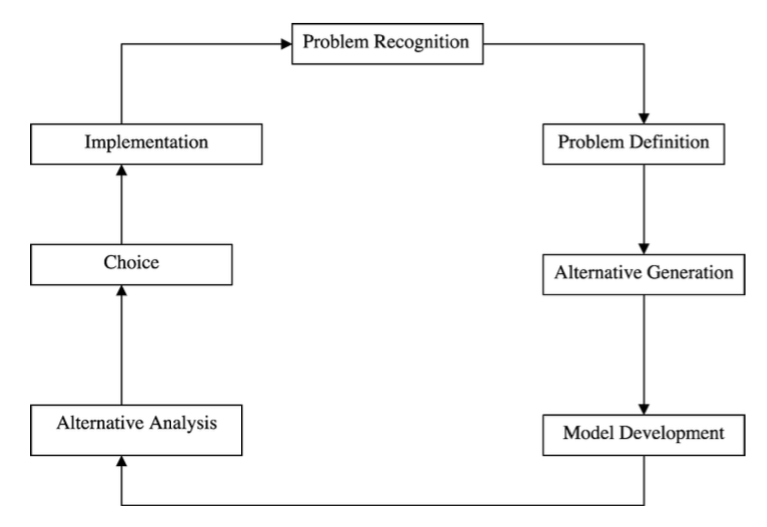
\includegraphics[scale=0.4]{Images/decisionSuppotProcess.png}
\caption[The DSS decision-making process]{The DSS decision-making process \cite{shim2002past}}
\end{figure}
\section{Types of DSS}
\label{sub:TypesOfDSS}
There exists a number of Decision Support Systems. These can be categorized into five types:
\begin{itemize} 
	\itemsep0em
	\item Communication-driven DSS  
	\item Data-driven DSS 
	\item Document-driven DSS 
	\item Knowledge-driven DSS 
	\item Model-driven DSS 
\end{itemize} 
We will explore each type briefly in the following sections.
\subsection{Communication-driven DSS}
\label{subsec:CommunicationDrivenDSS}
\indent A communication-driven DSS is a type of DSS that focuses on communication as well as help two or more users collaborate, share information, co-ordinate their activities and support shared decision-making.\cite{DDSTypes}The most common technology used to deploy this type of DSS is a web or client server. A few example of a communication-driven DSS include chats and instant messaging softwares, online collaboration and net-meeting systems or a simple bulletin board or threaded email.

\indent Communications-Driven DSS software should include at least one of the following characteristics:
\begin{itemize}
	\itemsep0em 
	\item Enables communication between groups of people
	\item Facilitates information sharing
	\item Supports collaboration and coordination between people
	\item Supports group decision tasks
\end{itemize}
% \paragraph{Group DSS}
% \label{subsubsubsec:GroupDSS}	
\textbf{Group Decision Support Systems(GDSS)} is a hybrid type of DSS. It is based on communication-driven DSS. Using various software tools, multiple users can work collaboratively in groupwork.\cite{DDSTypes}\\
Examples of group support tools are: 
\begin{itemize}
	\itemsep0em 
	\item Audio Conferencing
	\item Bulletin boards and web-conferencing
	\item Document Sharing
	\item Electronic Mail
	\item Computer Supported face-to-face meeting software 
	\item Interactive Video
\end{itemize}
\subsection{Data-driven DSS}
\label{subsec:DataDrivenDSS}
\indent Data-driven DSS is a type of DSS that is able to process huge amounts of data from different sources and store them in a data warehouse system. Data Driven DSS uses on-line analytical processing(OLAP) and Data mining techniques to extract the needed data which will be discussed in the section \textit{ToolsToDevelopDSS}. There exists two special purpose Data-driven DSS, they are: Executive Information Systems (EIS) and Geographic Information Systems (GIS). An example of a data-driven DSS is computer-based databases that have a query system.

\indent Executive Information Systems (EIS) are computerized systems intended to provide current and appropriate information to support executive decision making for managers using a networked workstation. They focus on graphical displays and on offering an easy to use interface that presents information from the corporate database. EIS offer strong reporting and drill-down capabilities.\cite{DDSTypes}

\indent A Geographic Information System (GIS) or Spatial DSS is a support system that represents data using maps. It helps people access, display and analyze data that have geographic content and meaning.\cite{DDSTypes}
\subsection{Document-driven DSS}
\label{subsec:DocumentDrivenDSS}
A relatively new field in Decision Support is Document-Driven DSS. Its focus is on the retrieval and management of unstructured documents. Documents can be Oral, written or video. They help a decision maker by keeping track of knowledge represented as documents that can affect the decisions.\cite{power2002building} Examples of oral documents are conversations that are transcribed; video can be news clips, or television commercials; written documents can be written reports, catalogs, letters from customers, memos, and even e-mail.\cite{DDSTypes}
\subsection{Knowledge-driven DSS}
\label{subsec:KnowledgeDrivenDSS}
Knowledge-Driven DSS can suggest or recommend actions to managers. It contains of specialized problem solving expertise also known as a knowledge base. The knowledge base comprises of rules, facts and procedures about a particular domain. The knowledge base also provides understanding of problems within that domain, and "skill" for solving some of these problems. A related technique used in knowledge-driven DSS is Data Mining, discussed in the section \textit{ToolsToDevelopDSS}. Intelligent Decision Support methods are used to build Knowledge-Driven DSS  \cite{power2002building}.
\subsection{Model-driven DSS}
\label{subsec:ModelDrivenDSS}
Model-Driven DSS (MDS) are a standalone systems that performs modeling of unstructured problems with an easy to use user interface. The most basic modeling functionality; the what-if model ;can be achieved using a simple statistical and analytical tool. There can exist a hybrid DSS system that combines the modeling functionality of the MDS and the complex analysis of data of an OLAP system.\cite{DDSTypes} In general, model-driven DSS uses complex financial models, simulation models, optimization models or multi-criteria models to provide decision support.\cite{DDSTypes} Data and parameters are provided by decision makers to the Model-driven DSS to aid decision makers in analyzing a situation. Very large databases are not needed in Model-driven DSS as they are not usually data intensive.\cite{DDSTypes} Model-Driven DSS can also be called model-oriented or model-based decision support systems.

Model-driven decision support process can be divided into three stages: 
\begin{itemize}
	\item Formulation : A model is generated in a form that can be accepted in the model solver.\cite{shim2002past}
	\item Solution : Finding the solution of the model in an algorithm form.\cite{shim2002past}
	\item Analysis : Analyze and interpret 'what-if' model solution or a set of solutions.\cite{shim2002past}
\end{itemize}

Initially optimization of Model-driven DSS focused on optimizing the solution algorithm, but later the focus shifted to also finding better techniques to formulate and analyze the functions to support the DSS.\cite{shim2002past}

Tools used in Model-driven DSS include \cite{makowski2003modeling}:
\begin{itemize}
	\item \textbf{Decision Analysis tools} - help decision makers decompose and structure problems. These tools aim to help a user apply models like decision trees, multi-attribute utility models, Bayesian models, Analytical Hierarchy Process (AHP), and related models.\cite{DDSTypes}
	\item \textbf{Forecasting Support System} - A computer-based system that supports users in making and evaluating forecasts. Users can analyze a time series of data.\cite{DDSTypes}
	\item \textbf{Linear Programming} - A mathematical model for optimal solution of resource allocation problems.\cite{DDSTypes}
	\item \textbf{Simulation} - A technique for conducting one or more experiments that test various outcomes resulting from a quantitative model of a system.\cite{DDSTypes}
\end{itemize}
\section{Tools to Develop DSS}
\label{sec:ToolsToDevelopDSS}
As Mentioned in the previous section, there exists a number of tools that are used to support the decision making process. In this section, I will explain briefly each of them.
\subsection{Data Warehouse Systems}
\indent Data warehouse systems are systems that allow the manipulation of data by using either computerized tools customized for a specific task or general tools and operators that provide a certain functionality. A Data Warehouse is basically a database that is designed to support decision making in organizations. Data warehouses are structured to contain large amounts of data and handle rapid online queries and managerial summaries. According to Power\cite{power2007brief}, Data warehouse is a subject-oriented, integrated, time-variant, nonvolatile collection of data that supports the management's decision making process.
\subsection{On-line Analytical Processing}
\indent On-line Analytical Processing (OLAP) is a technique used to support the decision support functionality especially in Data-driven DSS. It is linked to analysis of large collections of historical data.\cite{DDSTypes} OLAP software is used for manipulating data from a variety of sources that has been stored in a static data warehouse. The software can create various views and representations of the data.\cite{DDSTypes} Three main features should be available in a software product for it to be considered an OLAP application. They are: 
\begin{itemize}
\item Multidimensional views of data
\item Complex calculations
\item Time oriented processing capabilities
\end{itemize}
\subsection{Data Mining}
\indent Data Mining helps in extracting useful information by finding patterns or rules from existing data to produce data content relationships. It is based on Artificial Intelligence techniques combined with statistical tools. This information is then used to predict future trends and behaviors which also makes it a very important technique when implementing a data-driven DSS.
\subsection{Web-based DSS}
\indent Web-based DSS can be defined as a computerized system that provides an easier and less costly way to deliver decision support information or decision support tools to a manager, business analyst or a decision maker using a Web browser. As shown in Figure 2.2, any Type of DSS can either be web-based and implemented using web technologies or local based(LAN-Based). However, the web  opened a gateway that allowed for the implementation of DSS with larger scopes, access to more users and most importantly rapid access to "best practices" analysis and decision-making frameworks. The result would be well-designed DSS in a company. Using a Web infrastructure for building DSS promotes more consistent decision making on repetitive tasks\cite{power2000web}.
\begin{figure}[H]
\centering
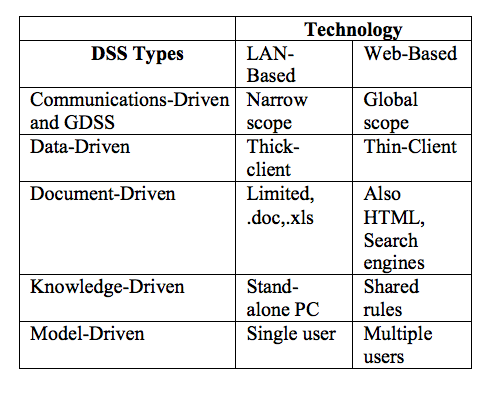
\includegraphics[scale=0.5]{Images/Web-based.png}
\caption[Decision Support Systems using Web Technologies]{Decision Support Systems using Web Technologies \cite{power2000web}}
\end{figure}
\section{DSS Design}
\label{sec:DSSDesign}
DSS has components and phases of development, like any other software system. No matter what kind of decision support system is being developed, there should exist four components:
\begin{itemize}
	\item Input: Input type that will be used in the analysis should be defined.
	\item User Knowledge/Expertise: will user knowledge be used as part of the input as well?
	\item Output: The output is specific or generic?
	\item Decisions: The system should suggest actions, analyze data and different actions or do the action to correspond to the output.
\end{itemize}
Once these four components are considered and clear enough we can proceed to the next phase in the design and development process which is Analyzing the business decision making process.

\subsection{Analyzing Business Decision Making Process}
A key consideration in designing a decision support system is to understand the context in which the decisions will be made. These considerations include the decision type, nature of problem, people involved and eventually the decision making context.\cite{DSS} An analyst is responsible for defining all the key components and creating a clear understanding of what will be required of the system.

Decisions can either be Strategic decisions, Operational decisions or Managerial decisions. It is very important to understand which type of decision should the DSS being developed support. 

Strategic decisions are non-repetitive and require a lot of time to be arrived at. They involve careful analysis of the situation and consequences. Some examples of strategic decisions: evaluation of an investment proposal, decisions related to mergers and acquisitions, resource allocations, fund raising, etc.\cite{DSS} Operational decisions can either be long term decisions that impact the business functionality and help the company realize their mission or short term decisions that impact day-to-day activities.\cite{DSS} Managerial decisions are usually decisions taken by top management. Examples of Managerial decisions include resource allocation, talent management, research and development, new product introduction, withdraw or revamp old products.\cite{DSS}

After defining the decision types to be supported, the nature of the problem should be defined. Problems can either be repetitive, non-repetitive, structured or unstructured and depending on the nature of the problem we can define what type of analysis will be required by the system and if any human interaction will be needed. Another factor to be taken into consideration is weather decisions are to be taken individually or within a group.

\subsection{Decision Making Process}
After analyzing the Decision making from a business perspective, the following step would be to start the decision making process. The process starts by the following steps:

\textbf{1. Defining the Problem}: It begins with recognizing that a problem exists, sets a base on which assumptions can be built, collect and analyze data and finally evaluate alternatives\cite{DSS}. A problem exists when:
\begin{itemize}
\item The expected output and the delivered output are different
\item There’s a divergence from the normal expected results
\item An action taken is not explainable
\end{itemize}

\textbf{2. Identifying Decision Maker}: A problem should be sent to the right person depending on its nature.\cite{DSS}

\textbf{3. Gathering Information} : A DSS can process tons of data in just few seconds thus helping the concerned person with collecting data and identifying the factors influencing the situation.\cite{DSS}

\textbf{4. Evaluating Alternatives and Deciding}: All possible courses of action are evaluated and the most suitable action is determined, by assessing the pros and cons of each alternative. A DSS helps in justifying a particular choice.\cite{DSS}

\textbf{5. Implementation and Follow-up}: Once the decision is taken, It’s time to implement the decisions. Decisions proposed should be monitored in order to determine weather it was helpful in achieving the objectives or not. If not the entire process must be repeated.
\section{Decision Support Implementation and Development}
Once There is a clear understanding of the system requirements and all the processes are defined and the design phase is complete, the development process begins. It starts with choosing a system development approach, followed by designing the user interface. The System Architecture, networking and security will be addressed in the \textit{DecisionSupportArchitecture} and \textit{DecisionSupportNetworkingAndSecurity} sections.\cite{DSS}
\subsection{Choosing a System Development Approach}
There are three common development approaches as shown below in Figure 2.3. Each of them will be discussed in detail.
\begin{figure}[H]
\centering
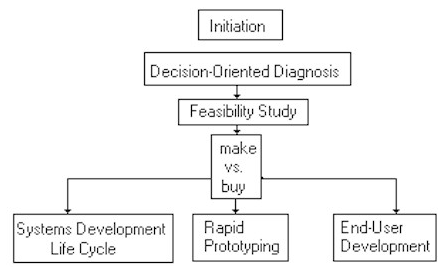
\includegraphics[scale=0.7]{Images/DSSDevelopmentApproaches.png}
\caption[DSS Development Approaches]{DSS Development Approaches \cite{DDSTypes}}
\end{figure}
\begin{itemize}
	\item \textbf{SDLC - System Development Life Cycle Approach}\\
	The SDLC is a sequential, structured and a standardized process for a system development. It starts with identifying the system objectives (needs of end users) and goes through various stages shown in figure 2.4\cite{SDLC}, including \\
	* System analysis (technical components required)\\
	* System design (architecture)\\
	* Development (programming)\\
	* Testing (errors and bug fixing)\\
	* Implementation \& Use(execution in the organization)\\
	* Evaluation (verification of functions and capabilities)\\
	* Modification (adjustments required)\\
\begin{figure}[H]
\centering
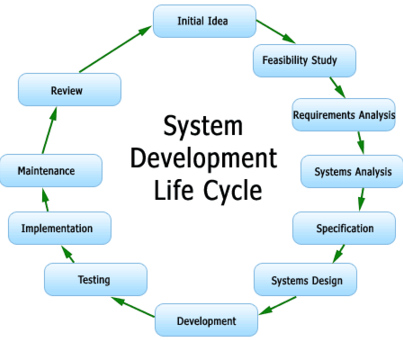
\includegraphics[scale=0.5]{Images/SLDC.png}
\caption[System Development Life Cycle Approach]{System Development Life Cycle Approach \cite{SDLC}}
\end{figure}
SDLC is the most commonly used and most rigid system development approach. In complex situations, it becomes difficult to use this approach, as the requirements of users are constantly changing. It doesn’t promote recurring development and testing.\cite{DSS}
	\item \textbf{Rapid Prototyping Approach}
Rapid Prototyping promotes a faster system development. It combines the effort of the decision makers and the analyst in charting the specific requirements. The decision maker uses general terms, the analyst uses DMS (database management system) to support rapid development of the application.\cite{DSS} Rapid prototyping goes through the following steps also shown in figure 2.5:\\
* Identifying objectives/ user requirements\\
* Developing the first model\\
* Evaluating the first model, identifying adjustments required and modification\\
* Testing the developed DSS. \\
* Go back to evaluation and modification, if needed\\
* Implementing\\
\begin{figure}[H]
\centering
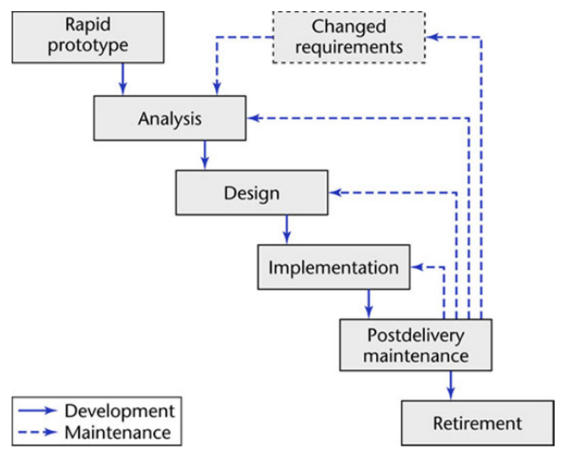
\includegraphics[scale=0.6]{Images/RPA.png}
\caption[Rapid Prototyping Approach]{Rapid Prototyping Approach \cite{RPA}}
\end{figure}
Evaluation and modification at a rapid pace is the core concept behind the Rapid Prototyping Approach as communication lines are always open. This approach is better suited than SDLC in complex situations.
	\item \textbf{End-User DSS Development Approach}
	Designing and development a software system depending on the specific or individual needs of the decision maker is the basis of the End-User development approach. The Decision maker customizes the system on his own. This approach is rarely used as usually the decision maker lacks technical expertise and chooses inappropriate software.\cite{DSS}
\end{itemize}
\subsection{Designing User Interface}
\label{subsec:DesigningUserInterface}
A Decision support system relies heavily on its design. If its user friendly and easy to use then chances are that this DSS will be used. Although the technical expertise of analysts, designers and developers is crucial, needs of DSS users must be evaluated and met at every step of the process. The right user interface design approach is the first step in developing an efficient decision support system.\cite{DSS}
\subsubsection{ROMC Design Approach}
ROMC is a systematic approach for developing large-scale DSS, especially user interfaces. The approach involves designing Representation, Operations, Memory Aids, and Control mechanisms. It is user-oriented approach for stating system performance requirements. It was originally presented by Sprague and Carlson in 1982.\cite{ROMC}

\textbf{Representation:} It involves presenting information or results, in a structured way.
All decision making activities in an organization take place in a certain environment or context. The representation in addition to the decision making context, provide a way to communicate information to the decision maker or user of the system about the situation.\cite{ROMC,DSS}. It provides a platform to the decision makers supported by information to help them interpret DSS outputs. It can be in the form of a table, graph, map, chart or a text document and each value on a map or a table communicates decision making context.\cite{ROMC,DSS}

\textbf{Operation: }Specific tasks that can be performed by a decision maker with a DSS. Example DSS operations include tracking market trends, carrying analytics or suggesting alternatives or performing all the functions.\cite{DSS}

\textbf{Memory Aid: }A data warehouse is the memory aid for a DSS. A DSS must give users a link to data warehouse. In addition, links and command shortcuts or sequences can be supplied to help users control a decision support system.\cite{DSS}

\textbf{Control Mechanism: }Allows users to effectively use representations, operations and memory aids.\cite{DSS}\\
% There exists some guidelines that should be followed by a Decision Support System user interface developer to ensure its usability\cite{DSS}:
% \begin{itemize}
% 	\item Get started with all significant information in hand. A DSS user interface developer must steer clear of assumptions and postulations. Rather he or she must rely on neat specifications.
% 	\item Be able to respond quickly to the needs of end users. A decision support system needs to be modified or evolved quickly as per the directions of the decision maker who is going to use the system. The designing of user interface should be such that it facilitates changes whenever required.
% 	\item Take into account the idiosyncrasies of the problems to be solved. Each DSS is developed to solve particular types of problems. Therefore, a user interface developer is expected to understand the peculiarity of the problems to be solved using DSS. And on the basis of this, he or she must be able to determine what kind of input a user must feed and how and what kind of output the system must produce.
% 	\item Pay attention to the order of priority while designing the software. This typically includes four steps. i) Design user interface, focusing on the dialogue that takes place between user and machine. ii) Design operations and commands that will be used to carry out the operations. iii) Define what happens when the user gives a command. iv) Work backward and create the program.
% \end{itemize}
\subsubsection{UI design success Factors}
In order to evaluate a UI design success. The following factors are considered:\\
\textbf{Execution Time} for a command given and action performed should be minimized.\\
\textbf{Versatility} of a decision support system should be flexible enough to integrate new tasks if needed.\\
\textbf{Adaptability} of a decision support system needs to remember the user's habits and adapt to them.\\
\textbf{Learning Time} should be reduced for the system.\\
\textbf{Uniformity of Command/theme} should be maintained throughout the system\\
\textbf{Quality of Help} should be available to users. The system should offer self-help manuals both online and offline.\\
\textbf{Memory Load;} Avoid too many numbers and statistical information on 1 screen. Users don't want to remember numbers\\
\textbf{Ease of Recall;} The user can remember how to use the system quickly after not using it for some time.\\
\textbf{Fatigue;} simple designs should be maintained to avoid Mental fatigue.\\
\textbf{Errors} should be managed for possible error-producing situations that might happen.
\section{Decision Support Architecture}
\label{sec:DecisionSupportArchitecture}
DSS Architecture requires full understanding of how a user will interact with the system and how the information will flow from one point to another.\cite{DSS} 
% What Does a DSS Architecture Scheme Address ?
% A well defined DSS architecture scheme addresses:

% A problem definition that a DSS is expected to resolve
% The objectives of a DSS
% Components of a DSS and connection between them
% Development and maintenance schedule
% Skills, tools, funds and other support required for DSS development
% Anticipated enhancements
% Project participants and their roles
There are four fundamental components of DSS architecture:
\begin{itemize}
	\item User Interface : Discussed in \textit{DesigningUserInterface}
	\item Database
	\item Model (context or situation representation)
	\item Knowledge
\end{itemize}

\textbf{Database: } A DSS accesses information directly from a database. The system architecture scheme focuses on the type of database required for a particular decision making system model, Who’s responsible for different types of databases and how to maintain accuracy and security of database.\cite{DSS}

\textbf{Model: }This component of the DSS architecture handles 2 components, the DSS model and DSS model management system. A model is a representation of a context, a situation or an event that carries out some type of data analysis needed for the decision making process. A DSS model management system stores and maintains DSS models.\cite{DSS}

\textbf{Knowledge: }Information about data relationship is represented in the knowledge. This knowledge is managed by the DSS architecture and provides decision makers with alternative solutions to a problem when needed.\cite{DSS} 
\section{Decision Support Networking and Security}
\label{DecisionSupportNetworkingAndSecurity}
DSS Network needs to define how hardware is organized, how data is distributed throughout the system how DSS components are connected and whether the information is fed/accessed using Internet, Extranet or Intranet.\cite{DSS} 
DSS Networking is all about connection between the components – software and hardware.

A network is defined as an assortment or a group of computers that are connected with each other or in a specific way, in order to communicate with each other. This connection facilitates the sharing of information among the connected computer systems.\cite{DSS}

\textbf{Resource Sharing}\\
The computer network's main objective is to share information. The most common technology for connection and resource sharing is LAN (Local Area Network). It serves hosts within a restricted geographical area. WAN (Wide Area Network) is another technology for resource sharing. The difference between LAN and Wan is that the latter is much larger and connects a group of LANs.\cite{DSS}

\textbf{Resource Connection}\\
TCP/IP (Transmission Control Protocol/ Internet Protocol) is a set of standard networking protocols, to enable computer systems to communicate with each other. It defines the rules and formats for the diffusion and reception of information or resources. The TCP sends data between programs using IP (Internet Protocol). It assigns a unique IP address to each workstation and sends information from one host to another in the form of packets.\cite{DSS}

Constant presence and cost effectiveness of the Internet make it the best way to send Information or data. One aspect that should always be taken into consideration is that data have to transferred through a secured connection to maintain security. Security related concerns are discussed in the next section.
\subsection{Security}
As a decision support system contains secret or classified information, it needs to be 100\% safe and secure. It’s also necessary for safeguarding employee and customer data.
The Process for Addressing Security Issues begins with:\\
\indent \textbf{Identifying security needs:} DSS users and analysts must brainstorm to identify security needs and evaluate potential threats.\\
\indent \textbf{Determining how important security is} for your DSS.\\
\indent \textbf{Remedying problems:}Fix the problems found that affect the DSS security. The solutions may be in the form of \cite{DSS}:\\
* Strengthened password\\
* User education\\
* Firewalls\\
* Enhanced privacy\\
* Logging and use statistics\\
\indent \textbf{Implementing solutions and observing their impact:} the decided solutions are implemented and observed.\\ 
There may be some security holes at any given point. DSS users and analysts must Keep track of them and change the passwords and strengthen firewalls on regular basis.
\section{Evaluation and Impact}
\label{sec:EvaluationAndImpact}
It is difficult to determine if a DSS is successful. Therefore, some criteria have to be evaluated and decided upon them how successful the system really is. Figure 2.6 shows a few examples of how various features of a DSS can be evaluated.\cite{Mysiak2005203} One aspect in evaluation of a DSS can be user satisfaction. However, users may have poor introspection or (if they are not experienced in using a DSS) may not recognize good advice and may dislike being corrected by a computer system, so while it should be taken into consideration, it shouldn't be a deciding factor.\cite{Mysiak2005203}
\begin{figure}[H]
\centering
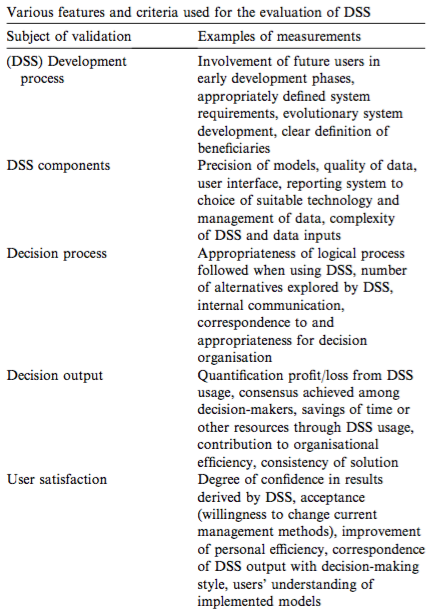
\includegraphics[scale=0.6]{Images/Evaluation_Features_DSS.png}
\caption[DSS Process Evaluation]{DSS Process Evaluation \cite{Mysiak2005203}}
\end{figure}
In addition to evaluating various DSS features, there exists some tools that can evaluate a DSS, Some of them include:\\
\textbf{1.Cost-Benefit Analysis:} Determines if a DSS is a good investment or not. This tool is used to compare the total benefits that a system is expected to produce vs the total cost of development and implementation .\cite{DSS} \\
\textbf{2.Incremental Value Analysis:} The process focuses on the value offered by a proposed DSS rather than the cost incurred on it.\cite{DSS}\\
\textbf{3.Qualitative Benefits Scenario Approach:} This method aims to determine if the proposed DSS will maintain the same quality and capabilities in future scenarios.\cite{DSS}\\
\textbf{4.Research and Development Options Approach:} This approach aims to determine the cost of keeping the DSS flexible for future enhancements or future DSS.\cite{DSS} \\
\textbf{5.Scoring Approach:} The approach separates the business and technical validation and considers other benefits of a DSS that were not considered during the analysis phase. It assigns points to each criterion/benefit upon reflecting on how well it satisfies a given factor.\\
\indent \textbf{Business validation} involves assessment of strategic alignment, management information support, competitive advantage and organizational risk.\cite{DSS} \\
\indent \textbf{Technical justification} involves examining technical uncertainty, strategic systems architecture and system infrastructure risk.\cite{DSS}